% ************************************************************************
%
% Introduction
%
% ************************************************************************
\chpos{22mm}{10mm}

\chapter[Introduction]{Introduction}
\markboth{\thechapter\ \ Introduction}{\thechapter\ \ Introduction}
\label{ch1:introduction}

%\mysquote{0.8\textwidth}{Quote text.}{Author (\oldstylenums{1000} - \oldstylenums{1100})}

%https://www.quantamagazine.org/why-the-first-drawings-of-neurons-were-defaced-20170928/
%https://www.npr.org/sections/health-shots/2017/01/26/511455876/art-exhibition-celebrates-drawings-by-the-founder-of-modern-neuroscience
%https://www.nytimes.com/2018/01/18/arts/design/brain-neuroscience-santiago-ramon-y-cajal-grey-gallery.html
%https://www.brainpickings.org/2017/02/23/beautiful-brain-santiago-ramon-y-cajal/
% The drawings 
\section{Need for neuron reconstruction}
\label{sec:neuron-cell}
\lettrine{F}{ascination} with neuronal cells dates back to the pioneering investigation over a century ago when a glance at a sample of silver-stained brain tissue disclosed the intricate network that forms the very essence of the nervous system. Remarkable milestone drawings of Santiago Ram\'{o}n y Cajal \cite{ramon2008histologia, swanson2017} -- the founding father of neuroscience -- remain as vivid as the digital images acquired by the newest fluorescence microscope. Ever since his breakthrough work, numerous studies \cite{ascoli2001computer, defelipe2002microstructure, defelipe1992pyramidal, van2001need, scorcioni2004quantitative, mason2007initiation, gensel2010semi, markram2015reconstruction} have explored the morphological features of neurons to gain deeper insight into their functionality, and the discipline gradually established as neuroscience \cite{kandel2000principles}. In the meantime, the astounding advancement of electrical engineering and computer science laid the foundation for more specialized disciplines such as neuroinformatics and neural engineering (Fig.~\ref{ch1:fig1}). Recently, attention has been directed towards brain science -- the field dedicated to the investigation of the captivating mechanism of, arguably, the most complex and enigmatic organ. The disclosure of Cajal's groundbreaking \textit{neuron doctrine}\footnote{Every neuron in the brain is a separate unit. Neurons conduct information in a defined direction and communicate across their synapses \cite{glickstein2006golgi}.} brought to light the idea that the nervous system is a network composed of building blocks called neuronal cells. Each cell (Fig.~\ref{ch1:fig2}) further represents a sophisticated, interconnected processing component that both transmits and processes the information. Different neuronal cells have different roles, and hence varying properties, including morphology, which offers useful evidences related to their functionality.

In the endeavor to understand neuron behavior and unravel the underlying principles, knowledge of neuronal cell morphology is essential for performing specialized analyses, which typically comprise the examination of changes in neuronal structure caused by external stimuli \cite{gomez2007immobilized, koppes2011neurite}, modeling \cite{ascoli2001computer}, statistical analysis \cite{samsonovich2005statistical, polavaram2014statistical}, describing connectivity patterns \cite{jiang2015principles}, branching patterns \cite{vallotton2007automated}, cataloging neuron phenotypes \cite{defelipe2013new}, classifying neuron types \cite{armananzas2015towards}, or simulating electrophysiological behavior. The morphology of a neuron can be captured to a high level of detail using microscopic imaging, but many studies require a more explicit representation than offered  by the resulting images, emphasizing the need for digital reconstruction of the morphology from the images into a tree-like graph structure. For example, the widely used Sholl analysis \cite{sholl1953dendritic}, commonly employed for quantification of the morphological characteristics of neurons \cite{garcia2014new}, is based on neuron reconstructions as a blue print of morphology. And numerous other neuroscientific studies directly rely on accurate knowledge of neuronal morphology in the form of digital reconstructions \cite{halavi2012digital, parekh2013neuronal}. This makes neuron reconstruction from microscopic images a highly important technical problem in the digital era of neuroscience \cite{peng2015diadem}.

\begin{figure}
	\begin{center}
		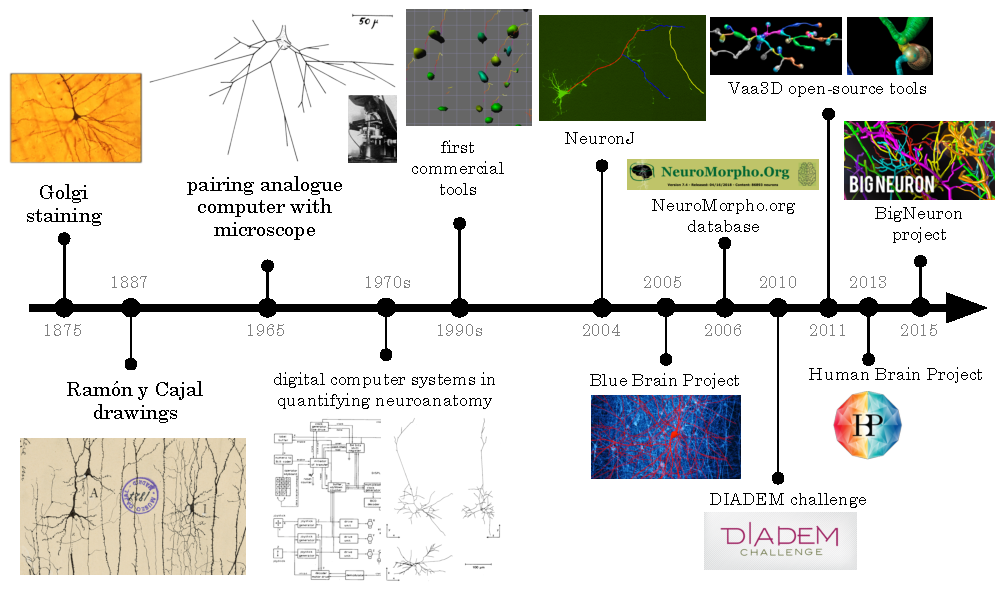
\includegraphics[width=\textwidth]{fig1}
	\end{center}
	\caption{Timeline overview of selected accomplishments related to neuron analysis. Advances in electrical engineering and computer science have been crucial for the great achievements in recent decades.}
	\label{ch1:fig1}
\end{figure}

Neuron reconstruction methodology has coevolved with technological advances in computing and imaging. With the early analogue computers \cite{glaser1965semi}, it became possible to connect a computer with a microscope and use analogue linear motion transducers to significantly speed up the gathering of information about the dendritic and axonal patterns. Subsequent generations of digital computers \cite{capowski1981accurate, capowski1977computer} brought further advances to neuron reconstruction by mixing computer graphics with the neuron image and using advanced operator controls such as a 3D joystick. The introduction of desktop PC hardware and software in the late decades of the 20th century increased the impact of computers \cite{halavi2012digital}, which by then were powerful enough to implement algorithms that, although previously developed, could not be directly run and shared between the users on a needed scale. It also marked the period when the first commercial and open-source academic software tools emerged (Fig.~\ref{ch1:fig2}). But with the ever growing amount and complexity of data, the quest for better solutions to neuron reconstruction continued. At present, even though many methods have been published and many tools are available, neurobiologists often still resort to manual or interactive approaches to get satisfactory results, indicating that reliable automated neuron reconstruction is a major challenge.

\section{Challenges in neuron reconstruction}
\label{sec:capturing-neuron}
The two crucial engineering tasks in neuron reconstruction are 1) reducing the time needed to obtain the reconstruction compared to manual delineation and 2) emulating or possibly surpassing the accuracy of the reconstruction compared to manual delineation. The astonishing increase in volume of microscopic imaging data rules out manual processing \cite{meijering2016imagining} and requires automated solutions that are fast enough to ensure high throughput in neuron analysis \cite{peng2017automatic}. Moreover, the wide variety of neurons and microscopic imaging modalities (dark-field, bright-field, confocal) puts high demands on automated processing \cite{svoboda2011past, peng2011proof}, and has resulted in a plethora of reconstruction methods \cite{peng2011automatic}. To date, two grand challenges have been organized in the field, namely DIADEM\footnote{http://diademchallenge.org} (short for digital reconstruction of axonal and dendritic morphology) and BigNeuron\footnote{http://bigneuron.org} \cite{peng2015diadem, peng2015bigneuron, gillette2011diademchallenge}, which aimed to stimulate community efforts to improve the state-of-the-art of neuron reconstruction. Despite great advancements, however, both engineering tasks still remain a major challenge. For instance, a 20-fold speedup compared to manual reconstruction has been projected \cite{liu2011diadem}, and proof-editing of automated reconstructions is still a bottleneck \cite{peng2011proof}.

\begin{figure}[t!]
	\begin{center}
		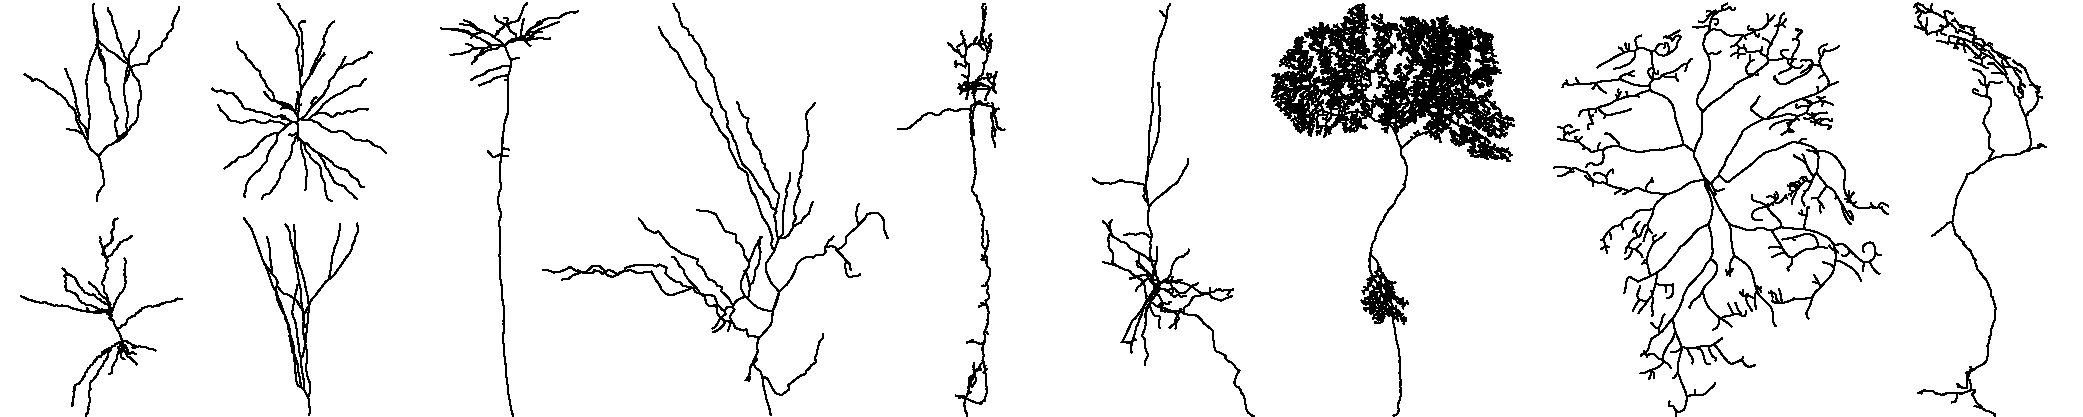
\includegraphics[width=\textwidth]{fig2}
	\end{center}
	\caption{Example neuronal arbors from NeuroMorpho.org showcase the morphological diversity across species, brain regions, and laboratories worldwide. The renderings were  exported using the web-based neuron morphology viewer \cite{bakker2016web}.}
	\label{ch1:fig2}
\end{figure}

In this thesis the focus is on detection and reconstruction of neurons from fluorescence microscopy images. Here, neurons are first labeled using a fluorescent dye in order to expose their structure, and then digital images are acquired using a light microscope, which are subsequently computer processed to reconstruct the morphology of the neurons. In practice, reconstruction algorithms often need to be customized to address a particular biological question or deal with a particular experimental condition, which may prevent them from being applicable across different experiments or laboratories. Key obstacles in achieving accurate and robust automation in neuron reconstruction \cite{meijering2010neuron, donohue2011automated, acciai2016automated} are the following:

1) The morphology of neurons is remarkably diverse (Fig.~\ref{ch1:fig2}) across brain regions and biological species. Even to expert human observers, the structural complexity of the neuronal arbors poses a significant challenge to visual comprehension, and manual delineation may easily take hours to days per neuron. This not only underscores once again the need for automation but also indicates that automated solutions require very powerful computer vision algorithms.

2) Neurons may be imaged using a variety of microscopy imaging modalities \cite{meijering2010neuron, donohue2011automated}. Each modality has its strengths and weaknesses, but all suffer from the diffraction limit, causing a blurring of structures below that limit as characterized by the point-spread function (\gls{psf}) of the microscope \cite{cox2012optical}, which under reasonable assumptions may be approximated by the Gaussian function \cite{zhang2007gaussian}. The diameters of dendrites and axons may vary significantly and be smaller (sub-$\mu$m) than the lateral resolution of the microscope. Moreover, the axial resolution is often even multiple times lower, further limiting the level of detail attainable in neuron reconstruction. Also, since neurons may have a relatively huge spatial extent compared to the field of view of the microscope, they are often imaged with lower magnification factors and thus larger voxel sizes, which limits the level of detail even more.

3) Eventually, all types of optical imaging are affected by photon noise \cite{van1998digital}, being a Poisson process. In accordance with earlier studies, the signal-to-noise ratio (\gls{snr}) of a microscope image is expressed as the ratio of the intensity inside a neuron above the background and the standard deviation of the noise inside the neuron \cite{cheezum2001quantitative, smal2010quantitative}. Depending on the illumination intensity and the fluorophore labeling density and homogeneity in an experiment, the SNR level may vary significantly between images, and even within one image. In addition, images may contain other types of background ``noise'', such as debris.

4) The ever increasing data volumes in neuron imaging counterbalance the increasing memory and processing speed of modern computers. Existing methods for neuron reconstruction often do not scale well with image volume size in terms of required processing time and accuracy \cite{peng2017automatic}. Dedicated engineering strategies to allow existing algorithms to reconstruct unlimited data volumes have been reported \cite{peng2017automatic, zhou2015neuron}, using data tiling approaches, but the challenge remains to develop algorithms that are not too adversely affected by image volume.

5) Evaluation of neuron reconstruction algorithms requires the availability of a reference or ``gold standard''. Reference reconstructions are typically obtained by expert manual annotation, which suffers from inter-observer and even intra-observer variability. Careful proof-editing \cite{peng2011proof} and making consensus reconstructions from multiple observers \cite{peng2015bigneuron} to improve the gold standard is extremely time consuming and not always feasible. Alternatively, synthetic neuron images may be used \cite{koene2009netmorph, radojevic2016fuzzy, radojevic-pnr}, whose true reconstructions are known by definition, but which are inevitably less realistic and less representative of the real problem. Thus, if the ultimate goal is to outperform humans in terms of both time and accuracy, new ways of evaluating algorithms are needed that do not depend as much on humans.

\begin{figure}
	\centering
	\begin{tabular}{c@{\hspace{1em}}c@{\hspace{1em}}c@{\hspace{1em}}}
		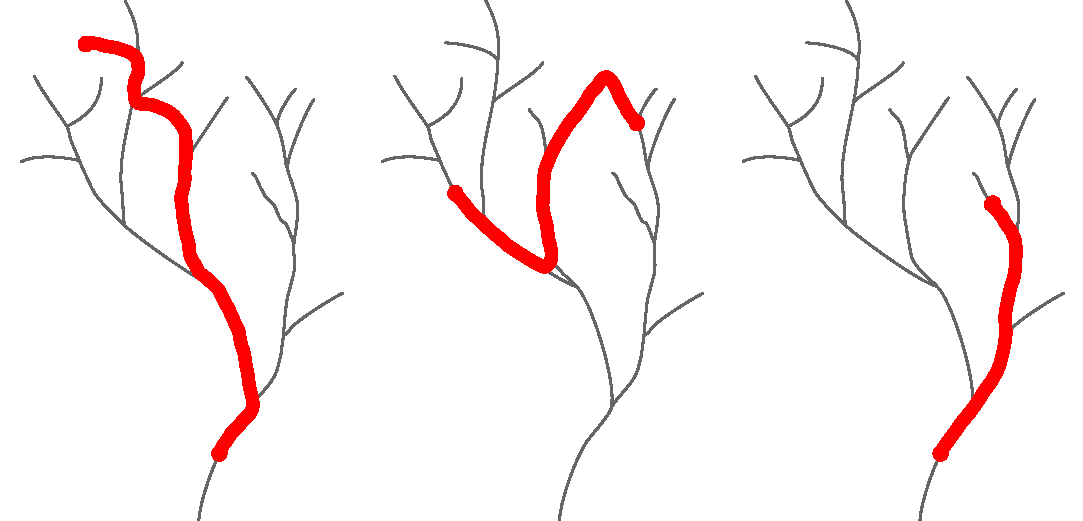
\includegraphics[width=0.3\textwidth]{fig3a} & 
		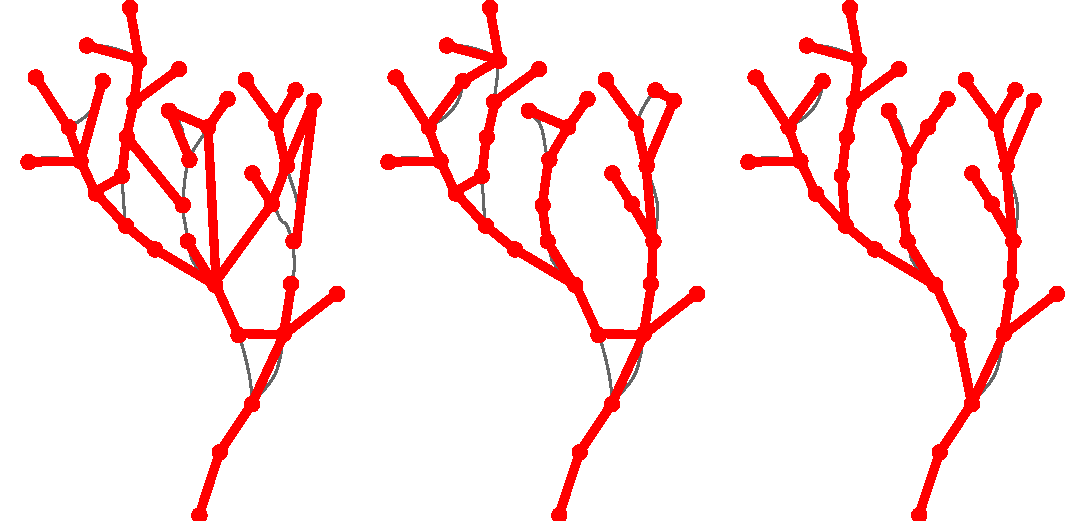
\includegraphics[width=0.3\textwidth]{fig3b} & 
		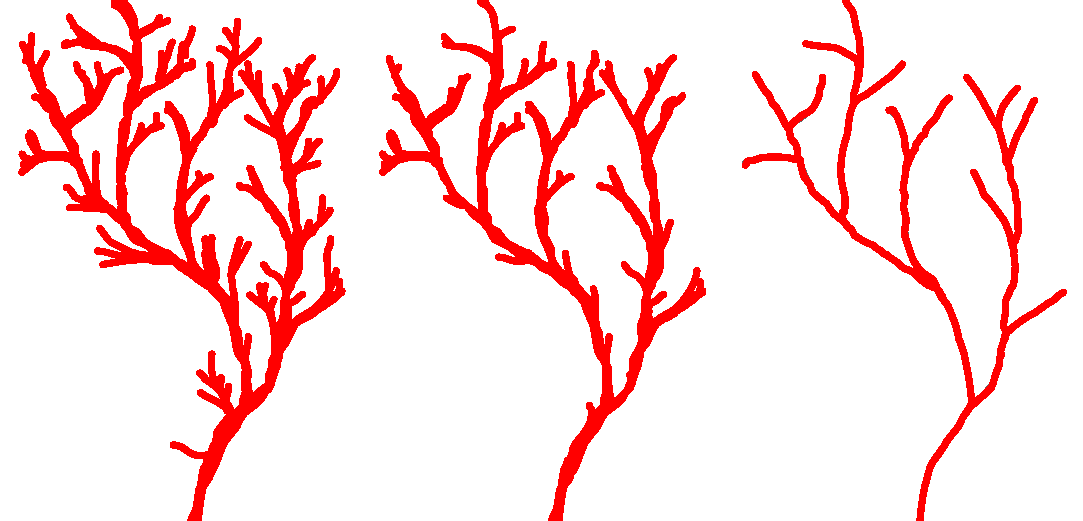
\includegraphics[width=0.3\textwidth]{fig3c} \\
		a) Shortest path tracing & b) Minimum spanning tree & c) Path-pruning
	\end{tabular}
	\caption{Common neuron reconstruction strategies. a) Finding an optimal path between any two control points. b) Inferring the optimal tree structure from a set of landmark points serving as nodes. c) Pruning an over-completely traced tree.}
	\label{ch1:fig3}
\end{figure}

\section{Common neuron reconstruction strategies}
\label{sec:reconstructions}
Single-cell neuron reconstruction methods typically employ different algorithmic approaches. The vast majority of works treats reconstruction as a modular task and uses a pipeline of different algorithmic units dedicated to processing particular tree components \cite{meijering2010neuron}. Nevertheless, there is inevitably a degree of commonality and interdependence among methods, as a cascade of processing units requires the output of one computation stage to be used in the next. Reconstruction accuracy also depends on the ability of a method to generalize well, which implies undertaking a fair share of global reasoning. The many methods introduced over the years \cite{meijering2010neuron, donohue2011automated, acciai2016automated} can be broadly cast into three categories of strategies (Fig.~\ref{ch1:fig3}), each involving various optimization tasks: 1) finding an optimal path between given control points (Fig.~\ref{ch1:fig3}a), 2) inferring an optimal tree from a set of given landmark points that already belong to the tree and that serve as its nodes (Fig.~\ref{ch1:fig3}b), and 3) pruning an over-traced and thus over-represented tree (Fig.~\ref{ch1:fig3}c). Of course, this categorization is not absolutely rigorous, and often the different strategies are combined.

Neuron branch tracing (Fig.~\ref{ch1:fig3}a) can be interpreted as an energy or cost optimization problem \cite{meijering2004design, peng2010automatic}. A classic example of this is to compute an optimal (``shortest'') path through the voxel grid, where the given geodesic metric or cost function is defined to weigh the transition between grid elements (graph vertices). This strategy has been used in many published methods \cite{meijering2004design, peng2010v3d, longair2011simple}, notably for semi-automated neuron tracing, where the control points are given by the user or are (interactively) computed from the image. Notable tracing approaches are geodesic shortest path \cite{peng2010automatic} or live-wire segmentation \cite{meijering2004design} solved using Dijsktra's shortest-path algorithm \cite{dijkstra1959note}. The downside of tracing defined in this manner is the necessity of having control points, which can be a challenge to obtain automatically and require global image reasoning. Computed traces can further be refined with energy optimization and solved using gradient descent algorithm \cite{peng2007straightening,peng2010automatic}.

The commonly used format to store reconstruction results (Section~\ref{sec:format}) assumes neurons to be tree-like structures consisting of connected nodes. Each two successive nodes constitute a neuronal branch compartment. Thus the essential geometrical quantities computed during tracing are the node center coordinates $\mathrm{p} = (x, y, z)$ and corresponding local (spherical) radii $r$ of the neuronal tree at those points. In addition the local direction $\mathrm{v} = ( v_x, v_y, v_z )$ at $\mathrm{p}$ may be computed. Taken together, a node is represented by a vector $\mathrm{x} = \left[  \mathrm{p}, r, \mathrm{v}\right]$, and a branch by a sequence of $N$ nodes $\mathrm{X} = \left\lbrace \mathrm{x}_1, \dots , \mathrm{x}_i, \dots, \mathrm{x}_N \right\rbrace$. The cumulative cost used by the optimization scheme to steer the tracing toward an optimal solution is computed over all nodes and compartments. Aside from geometrical constraints this typically also includes constraints based on image feature values such as local intensity or tubularity:
\begin{equation}
C(\mathrm{X}) = \sum\nolimits_{i} c(\mathrm{x}_i, I(\mathrm{x}_i)) \Delta\mathrm{x} 
\label{ch1_eq3}
\end{equation}
where the cost function $c$ could for example be decompose into:
\begin{equation}
c(\mathrm{x}, I(\mathrm{x})) = \alpha c_{\iota}(\mathrm{x}, I(\mathrm{x})) + (1-\alpha) c_{\gamma}(\mathrm{x}) 
\label{ch1_eq4}
\end{equation}
with $c_{\iota}$ denoting some intensity-based cost, $c_{\gamma}$ a geometry-based cost, and $ \alpha \in \left[ 0, 1 \right] $ a weight factor. The intensity-based cost could directly use intensities:
\begin{equation}
c_{\iota}( \mathrm{x}, I(\mathrm{x}) ) = I(\mathrm{x})
\end{equation}
or for example the exponential of the inverse intensity \cite{peng2010automatic}:
\begin{equation}
c_{\iota}( \mathrm{x}, I(\mathrm{x}) ) = \text{exp} \left(  \lambda  (1 - \tilde{I}(\mathrm{x}))^2 \right)
\end{equation}
where $ \tilde{I}(\mathrm{x}) = \tilde{I}(\mathrm{p}) = I(\mathrm{p}) / I_{\max}$, with $I_{\max} \equiv \max_{\substack{\mathrm{p}}} \left\lbrace  I(\mathrm{p}) \right\rbrace $, denotes normalized intensity. A popular alternative is to use:
\begin{equation}
c_{\iota}( \mathrm{x}, I(\mathrm{x}) ) = \rho(\mathrm{p})
\end{equation}
where $ \rho $ denotes some tubularity measure computed from the image intensities. If computed over a set of scales, it is written $\rho_{\Sigma}$, with $\Sigma = \left\lbrace \sigma_k \right\rbrace$, $1 \leq k \leq K$, and $\sigma_k$ denoting the individual scales. In particular the eigenvalues of the Hessian matrix computed at different scales are often used to measure the tubularity of local image structure \cite{sato19973d, frangi1998multiscale, steger1998unbiased, meijering2004design}. Tubularity measures are commonly computed at prefiltering stage and aim to reduce the presence of noise and non-tubular structures. They can be computed in an unsupervised manner, independent of the input data, or can be learned from the data in a supervised way \cite{sironi2016multiscale,li2017deep}, enabling adaption to a specific application based on the training. The downside of the latter approach, aside from having to design a suitable machine learning model, is that it requires dedicated training, which in practice can be time and resource consuming.

Trace refinement can be based on the discrepancy between the node positions and the centers of the local image intensity profiles. For example, to further align a trace to the underlying image intensities, the following cost could be minimized:
\begin{equation}
c_{\iota}(\mathrm{x}, I(\mathrm{x})) = \text{exp} \left( \lambda \frac{ \sum\nolimits_{\mathrm{y} \in \Theta(\mathrm{x})} \lVert \mathrm{x} - \mathrm{y} \rVert^2 I(\mathrm{y}) \Delta\mathrm{y}  }{\sum\nolimits_{\mathrm{y} \in \Theta(\mathrm{x})} I(\mathrm{y}) \Delta\mathrm{y} } \right) 
\label{ch1_eq2}
\end{equation}
where $\Theta(\mathrm{x})$ denotes a local spatial neighborhood of $\mathrm{x}$. Such refinement boils down to image intensity based mean-shifting \cite{cheng1995mean} of the node position, which can also be used to refine a collection of the overlapping tracings \cite{radojevic-pnr}. Alternatively, the zero-mean normalized cross-correlation (\gls{zncc}), which is independent of intensity offsets and scalings, can be used to quantify the similarity of the local image intensity profile and a theoretical model profile for trace refinement:
\begin{equation}
c_{\iota}(\mathrm{x}, I(\mathrm{x})) = \frac{ \sum\limits_{\mathrm{p} \in \Theta(\mathrm{x})} (I(\mathrm{p}) - \bar{I}(\mathrm{p}))(G_{\sigma}(\mathrm{p}) - \bar{G}_{\sigma}) }{ \sqrt{ \sum\limits_{\mathrm{p} \in \Theta(\mathrm{x})}(I(\mathrm{p}) - \bar{I}(\mathrm{p}))^2 \sum\limits_{\mathrm{p} \in \Theta(\mathrm{x})}(G_{\sigma}(\mathrm{p}) - \bar{G}_{\sigma})^2 } }
\label{ch1_eq1}
\end{equation}
where in this case $\Theta(\mathrm{x})$ typically is a cylindrical neighborhood of node $\mathrm{x} = [ \mathrm{p}, \sigma, \mathrm{v} ]$, centered at $\mathrm{p}$ with radius $\sigma$ and directed along $\mathrm{v}$, and $G_{\sigma}$ denotes the model profile at given scale $\sigma$, while $\bar{I}$ and $\bar{G}_{\sigma}$ are the respective mean intensity values of the image and the model inside region $\Theta$. In microscope images of neurons a reasonable choice for $G_{\sigma}$ is the Gaussian profile in the cross-sectional plane and the uniform profile in the axial plane of the cylindrical neighborhood \cite{radojevic2017neuron}. 

The geometry-based cost in (\ref{ch1_eq4}) can incorporate the vectorial (directional) alignment of nodes along the estimated tubularity direction \cite{meijering2004design}:
\begin{equation}
c_{\gamma}(\mathrm{x}) = c_{\gamma}(\mathrm{x}_{i}, \mathrm{x}_{i+1}) = \frac{1}{2} \left( \sqrt{1 - \varphi(\mathrm{p}_i, \mathrm{p}_{i+1})} + \sqrt{1 - \varphi(\mathrm{p}_{i+1}, \mathrm{p}_{i})} \right) 
\end{equation}
where $\varphi( \mathrm{p}_{i}, \mathrm{p}_{j} ) = | \mathrm{v}_i \cdot \mathrm{u}_{ij} | $ quantifies the alignment of the tubularity directions of two successive trace points with the unit link vector $\mathrm{u}_{ij} = (\mathrm{p}_j - \mathrm{p}_i) / \lVert \mathrm{p}_j - \mathrm{p}_i \rVert $ between them. Another example of a geometry-based cost is the trace smoothness \cite{peng2010automatic} or bending energy \cite{radojevic2016fuzzy} estimated using the second-order derivative:
\begin{equation}
c_{\gamma}(\mathrm{x}) = c_{\gamma}(\mathrm{x}_{i-1}, \mathrm{x}_{i}, \mathrm{x}_{i+1}) = \sum\nolimits_{i} (\mathrm{p}_{i-1} - 2\mathrm{p}_i + \mathrm{p}_{i+1})^2 \Delta\mathrm{p}
\end{equation}

Besides Dijkstra's shortest path algorithm, numerous other approaches to optimized local branch tracing have been reported. For example, energy optimization techniques such as active contours have been used to determine the optimal parametrized skeleton \cite{schmitt2004new}, or to directly find the open-curve representing a branch using gradient-vector flow to optimize the energy \cite{wang2011broadly}. Although path optimization methods require initialization in the form of control points, which can be a critical step, the use of active contours may refine even the initialization and improve the alignment of the control points to the local image context. The general downside of active contours, however, is the possibility of ending up with many discontinued branch segments due to gaps in low quality images. An alternative is to use the fast marching (FM) algorithm \cite{sethian1999level}. Conceptually similar to Dijkstra's shortest path algorithm, FM appears to be particularly useful for tracing curvilinear structures such as neuronal branches \cite{xiao2013app2, peng2011automatic, mukherjee2012automated, van2007subvoxel, santamaria2015automatic, basu2014reconstructing}, as it is able to bridge gaps. Particular implementations of FM-based neuron reconstruction, such as the APP2 method \cite{xiao2013app2}, have been very effective in reducing false-positives occurring in previous approaches \cite{van2007subvoxel, peng2011automatic}. Follow-up FM-based works have reported improvements in the speed of tracing discontinuous image structures by using gradient-descent combined with reinitialization \cite{mukherjee2012automated} and back-tracking \cite{liu2016rivulet}.

Accurately merging control points and any computed traces between them into a tree representation (Fig.~\ref{ch1:fig3}b) is a significant challenge due to the many possible alternatives to explore and evaluate. Since an exhaustive search for the optimal solution may require prohibitive amounts of computation time, the problem of assembling the many pieces of the neuron tree structure is often solved using approximations, but even so it remains an ongoing challenge \cite{peng2015bigneuron}. A significant share of the methods aims at finding a globally optimal solution, where the set of node candidates is turned into a weighted graph, and the reconstruction problem consists in extracting the optimal tree from this graph. One prominent method is the NP-complete\footnote{Non-deterministic polynomial-time.} minimum spanning tree (\gls{mst}) algorithm \cite{turetken2011automated, yuan2009mdl, gonzalez2010delineating, xie2010automatic}. A possible approach is to extract minimum trees spanning a subset of the graph's edges, but the solution to this problem is NP-hard \cite{chimani2009obtaining} involving plenty of exploration scenarios, and approximative solutions are used in practice \cite{blum2005combining, gonzalez2010delineating}. An alternative \cite{gonzalez2010delineating, xie2010automatic, turetken2011automated} is to find a k-minimum spanning tree (k-MST) spanning a subset of the graph's nodes (the control points) as opposed to the original MST spanning all nodes. Various criteria have been used with the MST algorithm to weigh and connect graph elements, for example based on distances and intensities \cite{yuan2009mdl}, or on probabilistic costs computed from the proximity of elements towards the middle of a filament \cite{turetken2011automated}. 

A particularly prominent family of methods is based on the pruning strategy (Fig.~\ref{ch1:fig3}c) to reconstruct neurons. Such methods start with an over-complete neuron tracing which is then gradually reduced (``pruned'') to converge towards an optimal concise representation of the neuronal tree. The underlying idea is to initially capture all voxels belonging to a neuron in a graph and subsequently to iteratively discard particular graph elements using various criteria. For example, in all-path pruning (\gls{app}) \cite{peng2011automatic}, over-complete traces are obtained using Dijkstra's algorithm, and the iterative pruning starts with the leaf nodes of the resulting graph. It executes in linear time, ensuring maximum coverage and minimum redundancy of the underlying neuron signal. Graph nodes that are already covered by others are removed with higher priority. A similar approach was employed in the follow-up work \gls{app2} \cite{xiao2013app2}, which introduced several improvements, such as the usage of a long-segment-first hierarchical pruning and dedicated preprocessing of the input image stack intended to optimize fast-marching based tracing.

\section{Neuron reconstruction using Bayesian filtering}
One of the main novelties proposed in this thesis to improve on commonly used neuron reconstruction strategies is the use of Bayesian filtering. Bayesian reasoning operates with the assumption that the states (quantities of interest) of any given system are not measurable directly but can be estimated (filtered) from observations using a recursive approach involving two essential processing steps: prediction and update \cite{doucet2001introduction}. More specifically, the unknown (hidden) states are expressed as a series of state vectors $ \left\lbrace \mathrm{x}_t; t \in \mathbb{N}, t \geq 0 \right\rbrace $ and are estimated in a probabilistic fashion using sequentially arriving independent observations $ \left\lbrace \mathrm{z}_t; t \in \mathbb{N}, t > 0 \right\rbrace $, leading to a  posterior distribution $p(\mathrm{x}_t|\mathrm{z}_t)$ of the states. This approach has been used extensively for tracking objects in sequential data (time series) in many applications \cite{ristic2004beyond, mahler2007statistical, stone2013bayesian, sarkka2013bayesian} but may also be applied to the problem of tracing neuronal branches in static data (spatial images). Here, the states could be defined as the node vectors $\mathrm{x} = \left[ \mathrm{p}, r, \mathrm{v}\right]$ introduced in the previous section, which are predicted and updated from one node to the next using Bayesian filtering. The actual state value $\hat{\mathrm{x}}$ of any given node may afterwards be estimated from the posterior distribution $p(\mathrm{x}|\mathrm{z})$ using for instance the maximum a-posteriori (MAP) approach or computing the centroid.

Formally, the joint posterior distribution of all state vectors up until (recursion) time $t$, that is $\mathrm{x}_{0:t} \equiv \left\lbrace \mathrm{x}_1, \mathrm{x}_2, \dots, \mathrm{x}_t \right\rbrace $, is obtained from corresponding observations, $\mathrm{z}_{1:t} \equiv \left\lbrace \mathrm{z}_1, \mathrm{z}_2, \dots, \mathrm{z}_t \right\rbrace $, by applying Bayes' theorem:
\begin{equation}
p(\mathrm{x}_{0:t} | \mathrm{z}_{1:t}) = \frac{p(\mathrm{z}_{1:t} | \mathrm{x}_{0:t}) p(\mathrm{x}_{0:t})}{\int p(\mathrm{z}_{1:t} | \mathrm{x}_{0:t}) p(\mathrm{x}_{0:t}) d\mathrm{x}_{0:t} }
\label{ch1_eq5}
\end{equation}
and the marginal distribution $ p(\mathrm{x}_t | \mathrm{z}_{1:t}) $ can be computed by recursively applying
\begin{equation}
\textrm{Prediction:} \quad p(\mathrm{x}_t | \mathrm{z}_{1:t-1}) = \int\! p(\mathrm{x}_t | \mathrm{x}_{t-1}) p(\mathrm{x}_{t-1} | \mathrm{z}_{1:t-1}) d\mathrm{x}_{t-1}
\label{ch1_eq6}
\end{equation}
\begin{equation}
\textrm{Update:} \quad p(\mathrm{x}_t | \mathrm{z}_{1:t}) = \frac{p(\mathrm{z}_t | \mathrm{x}_t) p(\mathrm{x}_t | \mathrm{z}_{1:t-1})}{ \int p(\mathrm{z}_t | \mathrm{x}_t) p(\mathrm{x}_t | \mathrm{z}_{1:t-1}) d\mathrm{x}_t}
\label{ch1_eq7}
\end{equation} 
The recursion mechanism uses a transition prior $ p(\mathrm{x}_t | \mathrm{x}_{t-1}) $, also called the transition model, to predict the next hidden state distribution from the previous, which allows to incorporate prior knowledge about state dynamics. And the predicted states are subsequently updated using the likelihood $ p(\mathrm{z}_t | \mathrm{x}_t) $, also called the observation model, which allows to incorporate prior knowledge about state appearance. Equations (\ref{ch1_eq6}) and (\ref{ch1_eq7}) can be rewritten more concisely as:
\begin{equation}
p(\mathrm{x}_t | \mathrm{z}_{1:t}) \propto p(\mathrm{z}_t | \mathrm{x}_t) \!\int\! p(\mathrm{x}_t | \mathrm{x}_{t-1}) p(\mathrm{x}_{t-1} | \mathrm{z}_{1:t-1}) d\mathrm{x}_{t-1}
\label{ch1_eq8}
\end{equation}
By custom design of the two models involved, the Bayesian filtering framework can be made to work for any given application, making it a fairly universal tool.

Several well-known analytical solutions to Bayesian filtering, such as the famous Kalman filter (KF) or hidden Markov model (HMM) filter, are based on mathematical assumptions that turn out to be very limiting in practice. For instance, the closed-form solution in the case of KF is based on the assumption that the models are linear and the distributions are Gaussian, which may not be accurate. Numerous other approximation schemes (extended KF, grid-based filters, et cetera) have been proposed with varying accuracy, practical feasibility, and computational cost. A popular alternative is  sequential Monte Carlo (\gls{smc}) filtering \cite{arulampalam2002tutorial}, in the literature also referred to as particle filtering (\gls{pf}), which has been used for a wide range of applications and is also the method of choice in this thesis. It approximates the posterior using discrete samples or particles\footnote{These terms are used interchangeably in the SMC-related content of this thesis.} and corresponding weights:
\begin{equation}
\left\lbrace \mathrm{x}_{t}^{(i)}, w_{t}^{(i)}; i = 1, \dots , N \right\rbrace
\label{ch1_eq9}
\end{equation}
so that the possibly intractable calculation of (\ref{ch1_eq8}) for non-linear and/or non-Gaussian cases is made tractable again. Here, $N$ denotes the number of samples, and using more samples generally leads to better approximation:
\begin{equation}
p(\mathrm{x}_t | \mathrm{z}_{1:t}) \approx \sum_{i=1}^{N} w_{t}^{(i)}\delta\big(\mathrm{x}_{t} - \mathrm{x}_{t}^{(i)}\big)
\label{ch1_approx}
\end{equation}
During SMC filtering, the weights are updated using a process known as sequential importance sampling (SIS), involving an importance function $\pi$:
\begin{equation}
w_{t}^{(i)} \propto w_{t-1}^{(i)} \frac{p(\mathrm{z}_t | \mathrm{x}_{t}^{(i)}) p(\mathrm{x}_{t}^{(i)} | \mathrm{x}_{t-1}^{(i)} )}{ \pi(\mathrm{x}_{t}^{(i)} | \mathrm{x}_{0:t-1}^{(i)}, \mathrm{z}_{1:t}) }
\label{ch1_eq10}
\end{equation}
One problem with SIS is the possibility of weight deterioration over time, leading to particle degeneration and a very sparse particle distribution, as a consequence of which the approximation fails to accurately represent the posterior. This can be avoided by regular resampling of the posterior distribution so that particles having higher importance weights remain more numerous.

% https://www.neuron.yale.edu/phpBB/viewtopic.php?t=3477
% http://www.neuromorpho.org/myfaq.jsp (What is SWC format?)
% http://research.mssm.edu/cnic/swc.html
% http://www.neuronland.org/NLMorphologyConverter/MorphologyFormats/SWC/Spec.html
\section{Neuron reconstruction tools and formats}
\label{sec:format}

Reconstruction software is nowadays implemented in a wide range of programming languages on different computer platforms and distributed over all regularly used operating systems \cite{meijering2010neuron, acciai2016automated}. The work presented in this thesis focuses on Java implementation within the ImageJ platform \cite{abramoff2004image, longair2011simple, pool2008neuritetracer} and on C++ implementation for the Vaa3D platform \cite{peng2014extensible}. Both platforms are widely used in bioimage analysis and thus facilitate deployment of the proposed methods. The latter is also the base platform for the BigNeuron project and provides various means to evaluate and benchmark neuron reconstruction methods. Evaluation is commonly carried out by comparing the reconstructed neuron tree with a gold standard reconstruction. In other words, measuring the performance of a neuron reconstruction method boils down to quantifying the resemblance of two graphs, one resulting from the method and the other typically from manual annotation of the image data. Resemblance is often computed in terms of internodal spatial distances but can also be based on a comparison of quantitative features computed from the graphs using tools such as L-Measure \cite{scorcioni2008measure} and BlastNeuron \cite{wan2015blastneuron}.

The most widely accepted format to store, exchange, and compare reconstructed neuron trees is the \gls{swc} format \cite{cannon1998line}, named after Stockley, Wheal, and Cole, who first described it \cite{stockley1993system}. It is an open-source space-delimited text format that stores tree structures as a list of nodes, $\mathcal{N} = \{ n_1, \dots , n_i, \dots , n_j, \dots  \}$, where each node contains certain properties related to the underlying neuronal geometry and topology. More specifically, each node in the SWC format, being a single line in the SWC file, contains seven attributes: node index identifier $i$, node type (soma, dendrite, axon, et cetera), three spatial coordinates $(x_i,y_i,z_i)$, radius $r_i$, and a parent node index (Fig~\ref{ch1:fig4}). By convention the latter is set to $-1$ for the origin node. To conform with a tree structure, each node $n_j$ may have only one parent $n_i$, with lower node index ($i<j$). Loops and disconnected branches should not exist as that would violate the tree-like structure. Even though there exist some variations of the SWC format, especially concerning the definition of the soma node\footnote{http://research.mssm.edu/cnic/swc.html}$^,$\footnote{http://www.neuronland.org/NLMorphologyConverter/MorphologyFormats/SWC/Spec.html}$^,$\footnote{NeuroMorpho.org FAQ: What is SWC format? http://www.neuromorpho.org/myfaq.jsp} for which the simple spherical model may not be suitable \cite{bakker2016web}, it is straightforward to implement and use, which explains its widespread adoption in many neuron morphology projects \cite{ascoli2007neuromorpho, peng2015bigneuron}. Some reconstruction methods are even based directly on the SWC format \cite{feng2015neutube}. The work described in this thesis uses  exclusively the SWC format.
 
\begin{figure}
\begin{center}
	\begin{tabular}{@{}c@{\hspace{1em}}c@{\hspace{0.25em}}c@{\hspace{2em}}c@{}}
	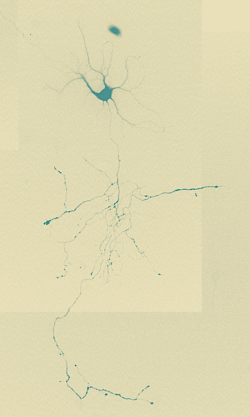
\includegraphics[align=c,width=0.2\textwidth]{fig4a} & 
	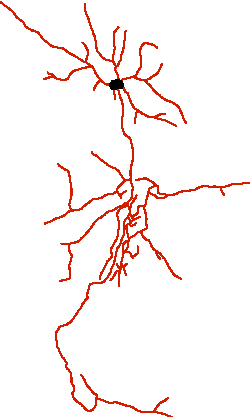
\includegraphics[align=c,width=0.2\textwidth]{fig4b} & 
	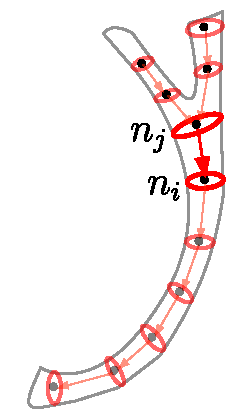
\includegraphics[align=c,width=0.2\textwidth]{fig4c} &
	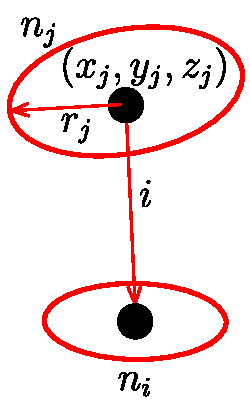
\includegraphics[align=c,width=0.2\textwidth]{fig4d} \\
	& & & \\[1ex]
	a) & b) & c) & d)
\end{tabular}
\end{center}
	\caption{Neuron morphology representation from image to digital reconstruction data format. a) Single neuron image. b) Digital reconstruction of the neuron exported using the web-based neuron morphology viewer \cite{bakker2016web}. c) Illustration of the SWC format as a list of nodes $n_i$. d) Detailed visualization of one segment (truncated cone) constituted by two connected nodes $(n_i, n_j)$ and basic node attributes.}
	\label{ch1:fig4}
\end{figure}

\section{Thesis outline and contributions}
\label{sec:outline}
This thesis addresses the need for further automation of neuronal image analysis. It presents methodological contributions and experimental results obtained while investigating computer vision solutions to various problems in extracting useful information from microscope images of single neuronal cells. The chapters propose original approaches to problems such as the detection of landmarks (critical points) of the neuronal tree, complete tracing and reconstruction of the tree, and the detection of regions containing neurons in high-content screens. Each chapter describes the proposed method, its software implementation, and evaluation. The remainder of this section gives a brief outline of the thesis and its contributions.

In Chapter~\ref{ch2:fuzzy} a new method is presented to detect critical points such as junctions and terminations of the neuronal tree in the images. A junction is loosely defined as a point where three branches merge, and a termination corresponds to a point where a branch ends. The proposed detection method uses directional filtering to extract essential features at every point in an image which are stored in linguistic terms and subsequently processed using fuzzy logic and rule-based reasoning to classify the point as background or a specific type of critical point. A custom-tailored set of IF-THEN rules is proposed for this purpose. The very concept of fuzzy sets allows points to have partial class memberships and thus helps to cope with uncertainty in the data. Defining a set of rules that can be truthful \textit{to a degree} is a convenient approach to fusing information into an aggregated decision.

In Chapter~\ref{ch3:phd} the Bayesian filtering framework is harnessed in a novel way to perform tracing of neuronal branch centerlines. The proposed method is based on probability hypothesis density (\gls{phd}) filtering to allow simultaneous tracing of an a priori unknown number of branches of the neuronal arbor. This specific type of filtering extends probabilistic tracing to the next generalization level and is implemented using \gls{smc} estimation. Compared to other works the present application differs fundamentally in the sense that the filtering is applied in space instead of in time. To make this work, new transition and observation models are proposed, incorporating prior knowledge about the shape and appearance of neurons in microscope images. Since the method is probabilistic, multiple runs may yield slightly different traces, providing accumulating evidence about the neuronal structures. This is helpful in the case of structural ambiguities in the images. The experimental results show this strategy indeed leads to more accurate tracings.

In Chapter~\ref{ch4:pnr} the probabilistic tracing idea is extended to a new automatic method for full neuron reconstruction. The method, named probabilistic neuron reconstructor (PNR), starts by identifying regions in the image that are highly likely to be neuronal branches according to a given tubularity measure, and seed points are then extracted from these regions to initiate the tracing process. Continuing the line of thought in the previous chapter, the method uses SMC estimation to perform probabilistic over-tracing of the neuronal arbor, resulting in multiple traces per branch to accumulate evidence about their morphology, including local branch diameters. Since the very idea of over-tracing is to collect statistically independent pieces of evidence, the tracing process from each seed point can be run independently, which in principle allows for straightforward parallelization to speed up the computations. To obtain the full reconstruction, the traces are refined and grouped into a single trace per branch, from which a tree representation is obtained using breadth-first search. An early version of the PNR method was a contender in the BigNeuron benchmark, where it already performed quite well. The method presented in this chapter is a substantially redesigned and improved version of it.

Lastly, in Chapter~\ref{ch5:ndetchml}, a feasibility study is presented of detecting neurons in high-content images of cell cultures from screening studies. The considered task is typically the first step in a high-throughput analysis pipeline, where regions containing neurons are detected in large image mosaics of low resolution but wide field-of-view, which can subsequently be scanned in high resolution for further morphological analysis using methods such as presented in the previous chapters. The detection is performed using supervised machine-learning methods trained on a very large number of image features. The considered machine-learning methods include support vector machines, random forests, k-nearest neighbors, and generalized linear model classifiers, and the image features are extracted using the compound hierarchy of algorithms representing morphology (CHARM) and the scale-invariant feature transform (SIFT). The experimental results indicate that a random forests classifier using the right feature subset ranks best but is not statistically significantly better than some of the support-vector machine based classifiers. A pilot with deep-learning based artificial neural networks shows that the traditional classification methods are yet to be preferred given the limited available data and annotations.